\section{Information value depends on available actions}

E6 crosses signal information with action-set flexibility in three constructive environments. Define the interaction as the difference-in-differences between informative and uninformative signals under flexible and restricted action sets. Ignoring a signal remains feasible, so information value is non-negative in each action set; exact ignore-signal anchors and signal-garbling checks verify this implementation invariant.

The interaction spans all three theoretically admissible cases (Fig.~\ref{fig:information}). When flexibility unlocks state-contingent specialization, the estimate is \EsixPositive{} with 95\% family-wise interval \EsixPositiveLow{} to \EsixPositiveHigh{}. A robust fallback makes information and flexibility substitutes, giving \EsixSubstitution{} with interval \EsixSubstitutionLow{} to \EsixSubstitutionHigh{}. A dominated added option yields the exact-null interaction \EsixNull{}. All three intervals meet the precision criterion at \EsixReplications{} replications.

This sign pattern shows why information and flexibility are not universally complementary. Information is actionable when it changes a feasible contingent decision, but the incremental value of the signal depends on what the enlarged action set adds. E5 cross-law dependence diagnostics are therefore kept separate in Supplementary Fig.~S3: its experiment-level precision criterion was not met, so it cannot support a general claim about copula misspecification, regret or downside risk.

\begin{figure}[t]
\centering
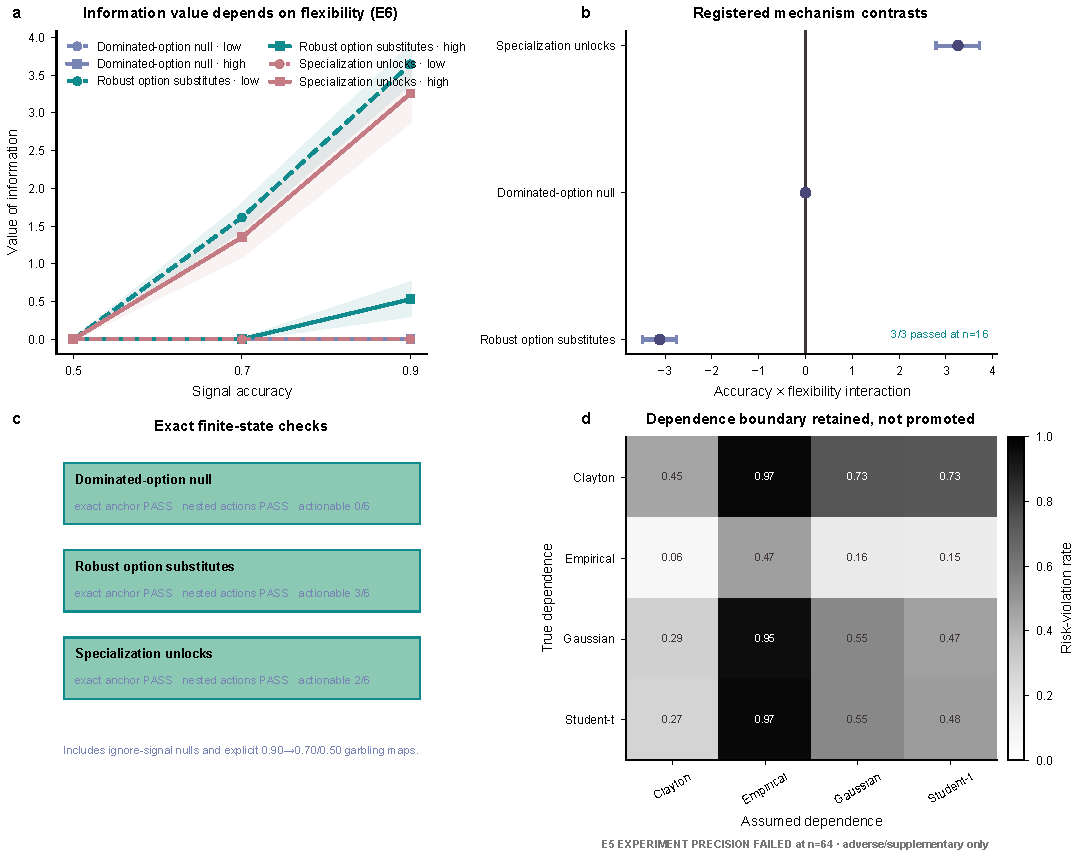
\includegraphics[width=\textwidth]{../figures/stage_ii/main/Figure5.pdf}
\caption{\textbf{Information and action-set flexibility can complement, substitute or be unrelated.} The E6-only display reports three registered archetypes, their interaction intervals, exact finite-state checks and archetype-specific flexibility gains. All three family-wise intervals meet the pre-specified precision criterion.}
\label{fig:information}
\end{figure}
